%!TEX program = pdflatex
% Full chain: pdflatex -> bibtex -> pdflatex -> pdflatex
\documentclass[11pt,en,cite=authoryear]{elegantpaper}
\usepackage{float}
\title{Project 5 \& Project 9 report}
\author{Xiaolin Zhang \\ 2019xxxxxx xxxxxxx \and Ziyang Xu \\2019xxxxxx xxxxxxx  \and Wangzhihui Mei \\ 2019124044 6603385  \and Xiaohuan Pei \\ 2019xxxxxx xxxxxxx}
\institute{CCNU-UOW JI}

% \version{0.09}
\date{}

% cmd for this doc
\usepackage{array}
\newcommand{\ccr}[1]{\makecell{{\color{#1}\rule{1cm}{1cm}}}}

\begin{document}

\maketitle

% \begin{abstract}
% This documentation illustrates the usage of the \href{https://github.com/ElegantLaTeX/ElegantPaper}{ElegantPaper} template. This template is based on the standard \LaTeX{} article class, which is designed for working paper writing. With this template, you can get rid of all the worries about the format and merely focus on writing. For any question, please leave a message on \href{https://github.com/ElegantLaTeX/ElegantPaper/issues}{GitHub::ElegantPaper/issues}. Want to know more about Elegant\LaTeX{} Templates? Please visit: \href{https://github.com/ElegantLaTeX}{https://github.com/ElegantLaTeX}.\par
% \keywords{Elegant\LaTeX{}, Working Paper, Template}
% \end{abstract}

\section{Project 5}
\subsection{Dataset: Artificial Characters Learning Problem}

This database has been artificially generated by using a first order theory which describes the structure of ten capital letters of the English alphabet and a random choice theorem prover which accounts for etherogeneity in the instances. The capital letters represented are the following: A, C, D, E, F, G, H, L, P, R. Each instance is structured and is described by a set of segments (lines) which resemble the way an automatic program would segment an image. 


Each instance is stored in a separate file whose format is the following:
\begin{lstlisting}
CLASS OBJNUM TYPE XX1 YY1 XX2 YY2 SIZE   DIAG
1     0      line 0   0   0   13  13.00  45.28
1     1      line 20  0   22  15  15.13  45.28
1     2      line 0   13  22  15  22.09  45.28
1     3      line 0   13  0   27  14.00  45.28
1     4      line 22  15  23  39  24.02  45.28
1     5      line 0   27  23  39  25.94  45.28
\end{lstlisting}

\begin{figure}[h]
	\centering
	
\includegraphics[width=0.5\textwidth]{image/chars}
	\caption{The generated characters}
	\label{chars}
\end{figure}

where CLASS is an integer number indicating the class as described below, OBJNUM is an integer identifier of a segment (starting from 0) in the instance and the remaining columns represent attribute values. \cite{schapire1999improved}.

The generated character image is like Figure \ref{chars}


\subsection{Data pre-process}
The character described by segments is represented as the vertex pair, we transform them to binary grid ($12\times 8$), like Figure \ref{transform}.

\begin{figure}[h]
	\centering
	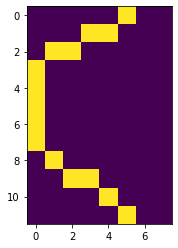
\includegraphics[width=0.3\textwidth]{image/C_array}
	\caption{The representation of "C"}
	\label{transform}
\end{figure}

Then the problem is transformed into one like the MNIST classification problem. The feature is the flattened 0-1 pixel, whose dimension is $96\times 1$, the label is "A", "C", "D", "E", "F", 
"G", "H", "L", "P", "R", which correspond to the numbers 0 through 9. 


We got 6000 training data from the primitive dataset. We shuffled them and use 70\% of the data as training data, 30\% as test data. The label distribution of training data is like Figure \ref{dist_y}

\begin{figure}[h]
	\centering
	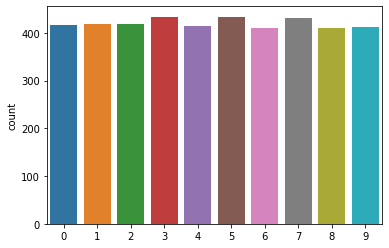
\includegraphics[width=0.4\textwidth]{image/dis_y}
	\caption{The label distribution of training data}
	\label{dist_y}
\end{figure}


\subsection{Model construction}
\subsubsection{Ensembling Model}
Ensemble modeling is a process where multiple diverse models are created to predict an outcome, either by using many different modeling algorithms or using different training data sets. The ensemble model then aggregates the prediction of each base model and results in once final prediction for the unseen data. The motivation for using ensemble models is to reduce the generalization error of the prediction. As long as the base models are diverse and independent, the prediction error of the model decreases when the ensemble approach is used. The approach seeks the wisdom of crowds in making a prediction. Even though the ensemble model has multiple base models within the model, it acts and performs as a single model. Most of the practical data mining solutions utilize ensemble modeling techniques. Chapter 4 Classification covers the approaches of different ensemble modeling techniques and their implementation in detail.

In this task, We applied Voting method. Voting is a combination strategy for classification problems in integrated learning. The basic idea is to select the most output class among all machine learning algorithms.

There are two types of output of classification machine learning algorithms: one is to directly output class labels, and the other is to output class probabilities. Using the former to vote is called hard voting (majority/hard voting), and using it to classify is called soft voting (Soft voting). VotingClassifier in sklearn is the implementation of voting method.

In this project, We compared hard voting classifier and soft voting classifier, and got better performance in hard voting classifier, which ensemble Logistic Regression, SGD, SVM, Decision Tree, Random Forest, Extra Tree, MLP as one classifier. The structure is like Figure \ref{vcl}.

\begin{figure}[h]
	\centering
	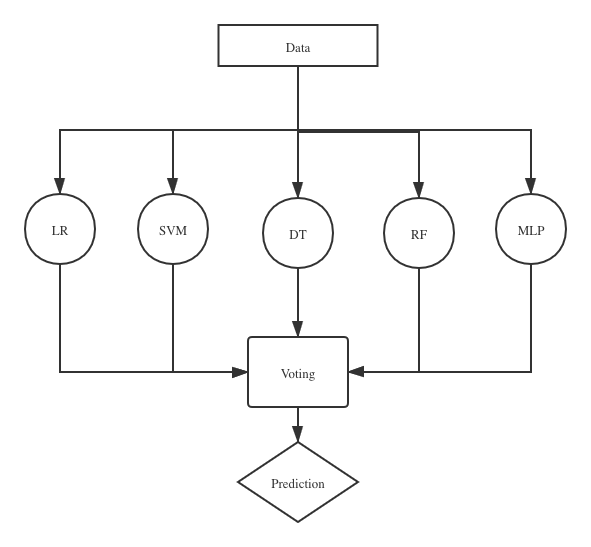
\includegraphics[width=0.5\textwidth]{image/voting}
	\caption{The Ensembled Voting classifier}
	\label{vcl}
\end{figure}

\subsubsection*{Performance}
We calculated the Recall, Precision, Accuracy and F1-score of the model. As this is a multi-class classification, so each label correspond to one micro value, we can calculate the mean of micro value and get marco value.
\begin{figure}[H]
	\centering
	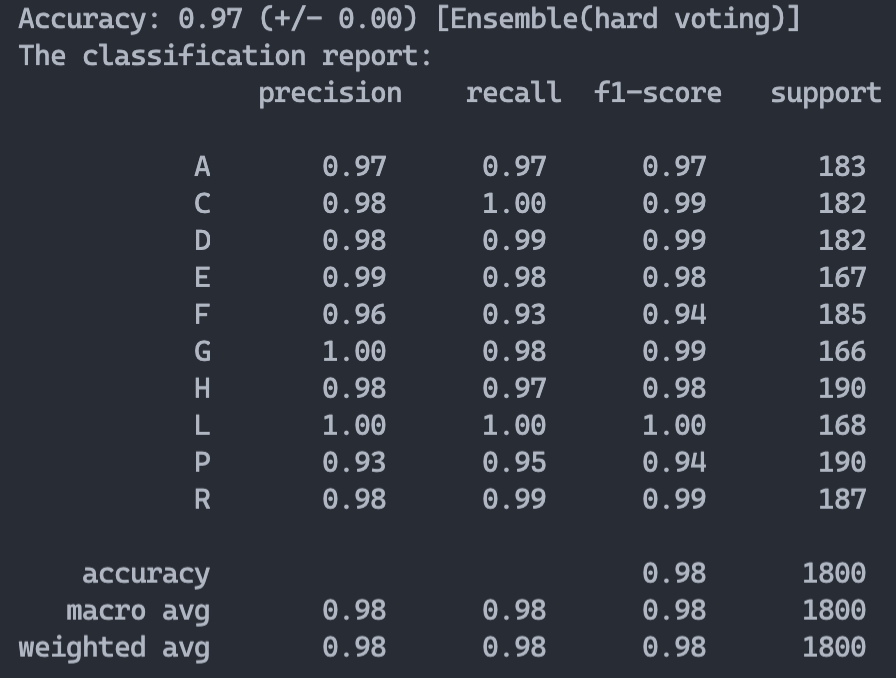
\includegraphics[width=0.6\textwidth]{image/hvpf}
	\caption{The Ensembling (Hard voting) performance}
	\label{hvpf}
\end{figure}
So, we can draw the conclusion that Ensemble Model perform well on both micro and marco f1-score.
\bibliography{wpref}
\end{document}
